%%=============================================================================
%% Methodologie
%%=============================================================================

\chapter{Methodologie}
\label{ch:methodologie}

%% TODO: Hoe ben je te werk gegaan? Verdeel je onderzoek in grote fasen, en
%% licht in elke fase toe welke stappen je gevolgd hebt. Verantwoord waarom je
%% op deze manier te werk gegaan bent. Je moet kunnen aantonen dat je de best
%% mogelijke manier toegepast hebt om een antwoord te vinden op de
%% onderzoeksvraag.
\section{Redenen}
\label{sec:Redenen}

TO DO (ook nog andere titel)

\section{ Technische voor-en nadelen van Puppet en Ansible}
\label{sec: technische-voor-en-nadelen-van-Puppet-en-Ansible}

\subsection{ Infrastructuur met Vagrant}
\label{sec: infrastructuur-met-Vagrant}

Zowel Puppet als Ansible hebben een gelijkaardige infrastructuur, maar verschillen in de details. Om de resultaten van deze vergelijkende proef zo betrouwbaar mogelijk te maken is getracht de verschillen tussen beide opstellingen zo minimaal mogelijk te houden. Beide opstellingen zijn dan ook gebasseerd op de infrastructuur die te zien is op afbeelding \ref{fig:infrastructuur}.

In het geval van Puppet zal server A uit afbeelding \ref{fig:infrastructuur} de PuppetMaster zijn. Het is deze server die de Puppet manifesten bewaart en compileert naar catalogussen. In het geval van Ansible zal op server A Ansible Tower ge{\"\i}nstalleerd zijn en verder bevat deze server uiteraard het Ansible equivalent van manifesten, playbooks genaamd. 

Server B t.e.m. D stellen de clients voor. Zij ontvangen een bepaalde configuratie van server A om vervolgens de nodige services te installeren en te configureren.

\begin{figure}
  \begin{center}
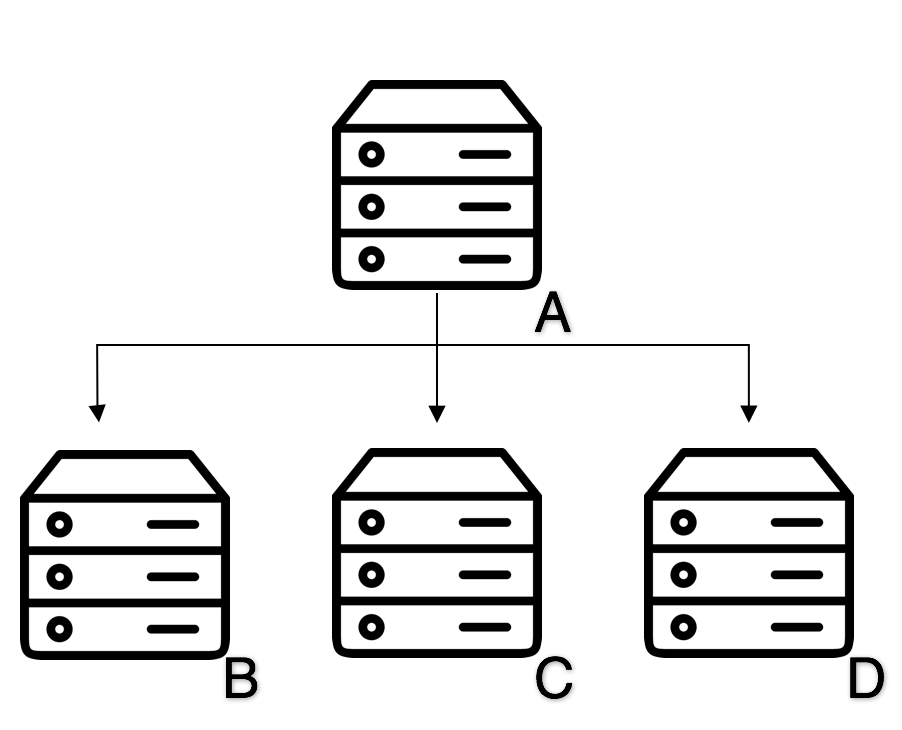
\includegraphics[width=150px]{img/infrastructruur.png}
\end{center}  \caption{Infrastructuur}
  \label{fig:infrastructuur}
\end{figure}

Om deze opstelling te kunnen verwezelijken en om gelijkheid tussen beide infrastructuren te garanderen wordt er gebruik gemaakt van Vagrant. Deze technologie maakt het mogelijk om op een eenvoudige manier herhaaldelijk dezelfde servers op te kunnen zetten. Vervolgens worden deze servers voorbereid met de nodige configuraties zoals het installeren van de monitoringstool. Het is vanzelfsprekend dat de monitoringstool al ge{\"\i}nstalleerd is alvorens Puppet en Ansible de configuraties van de servers overnemen, want het is juist dit dat gemeten dient te worden, de impact van Puppet en Ansible op deze servers en het netwerk. Daarom is er ook beslist om de configuratie van de monitoringstool ook door Vagrant te laten gebeuren, zodat de monitoringstool reeds operationeel is als Ansible en Puppet in werking treden. De vagrantfile om dit te verwezenlijken ziet er als volgt uit.


\underline{\textbf{Vagrantfile}} (Puppet infrastructuur)
\lstinputlisting[language=Ruby]{/Users/thomasdetemmerman/Documents/Bachelorproef-Ansible-vs-Puppet/ProofOfConcept/Puppet/Vagrantfile}

Een woordje uitleg bij deze Vagrantfile:

Lijn 1 en 2 zijn variabelen. 'AmountOfVM' stelt het aantal client VM's voor. In totaal zullen er dus altijd AmountOfVM + 1 virtuele machines aangemaakt worden. Deze '+ 1' is afkomstig van de master welke standaard aangemaakt wordt.

Lijn 6 t.e.m.19 betreffen de master VM, net als server A uit afbeelding  \ref{fig:infrastructuur}.
De reden van lijn 14 en 15 is om het probleem op te lossen waarbij de interface, die aangemaakt wordt op lijn 13, niet automatisch gestart wordt. 
Lijn 17 en 18 starten het script dat de nodige software installeert om deze server als PuppetMaster te laten opereren.

Lijn 22 t.e.m 37 betreffen de clients, net als server B, C, D uit afbeelding  \ref{fig:infrastructuur}. Dankzij de variable 'AmountOfVM' kunnen deze dynamisch bijgebouwd worden. 
Lijn 22 t.e.m 25 zorgen ervoor dat alle VM's dezelfde resources ter beschikking krijgen. Deze resources zijn bewust laag gehouden zodat fluctuaties in de monitoringstool beter waargenomen kunnen worden.
Lijn 33 en 34 zorgen voor de opstart van het script newrelicinfra.sh. Dit script installeert New Relic, de gekozen monitoringstool. Hiermee zijn we in staat om data van de VM  te analyseren vanop het online platform van New Relic.
Lijn 35 en 36 starten het script genaamd installpuppetagent.sh. Dit script bestaat uit de volgende stappen:

\underline{\textbf{installpuppetagent.sh}} 
\lstinputlisting[language=Ruby]{/Users/thomasdetemmerman/Documents/Bachelorproef-Ansible-vs-Puppet/ProofOfConcept/Puppet/puppetconfiguration/installpuppetagent.sh}

Hierbij wordt er eerst de repository van Puppet toegevoegd om vervolgens Puppet te installeren. Hierna wordt de bestaande 'hosts-file' vervangen  door een nieuwe. Dit is vanwege de afwezigheid van een DNS-server in onze opstelling. Ook wordt de Puppet.conf aangepast. Hierbij voegen we de FQDN van de PuppetMaster toe. Om te eindigen starten we de service en doen we een aanvraag bij de master voor een certificaat. Dit is nodig omdat zonder certificaat er geen vertrouwensrelatie bestaat tussen de master en de client. Bijgevolg kan er dan ook geen catalogus verstuurd worden naar deze client.


Ondanks het feit er getracht is geweest om de verschillen zo klein mogelijk te houden, blijven het verschillende technologie\"en. Hieronder is een lijst opgesomd van de lijnen die niet overeenkomen met Puppet.

\underline{\textbf{Vagrantfile}} (Ansible infrastructuur)\newline\newline

2 VmGroupName ="Anode" \newline
11 machine.vm.box ='ansible/tower' \newline
14  machine.vm.network "private\_network", ip: "192.168.100.20" \newline
17  \#NIET AANWEZIG\newline
18  \#NIET AANWEZIG\newline
29  machine.vm.network "private\_network", ip: "192.168.100.\#\{20+machine\_id\}"  \newline
35  \# NIET AANWEZIG\newline
36 \#NIET AANWEZIG\newline

De afwezigheid van lijn 17 en 18 bij Ansible is te wijten aan het feit dat de installatie van Ansible Tower vervat zit in de vagrantbox op lijn 11. Verder is het opmerkelijk dat ook lijn 35 en 36 niet aanwezig zijn. Dit is dan ook een eerste belangrijk verschil dat al in deze vroege fase duidelijk wordt. Namelijk de afwezigheid van het script installpuppetagent.sh. Dit script zorgt voor de installatie van de Puppetagent op de clients. Aangezien Ansible geen gebruik maakt van agenten is een dergelijk script ook niet aan de orde.






















